% !TEX root = ../thesis.tex

\chapter{Výsledky testovania technológií}
\label{evaluation}

V tejto kapitole je zhrnuté porovnanie testovaných scenárov a postupov na nasadenie platformy Kubernetes a Kubeflow, ktoré sa využívajú na riešenie problémov strojového učenia. Priblížené sú problémy, ktoré sa vyskytovali pri uplatňovaní týchto plánov, ich zvládnutie, objektívne vyhodnotenie týchto technológii a vyzdvihnutie najlepšieho spôsobu.

Testovanie prebiehalo na serveroch od portálu CLOUD TUKE s operačnými systémami Windows server 2019 a Ubuntu 20.04 Desktop s nasledovnými parametrami:

\begin{itemize}
	\item Procesor: \textbf{Intel(R) Xeon(R) CPU E5-2670 v3 @ 2.30GHz}
	\item Počet jadier: \textbf{8}
    \item Veľkosť operačnej pamäte RAM: \textbf{16GB}
    \item Veľkosť pamäťového úložiska: \textbf{70 - 100GB}
\end{itemize}

Pre menej náročné scenáre bol tiež využívaný osobný laptop s operačným systémom Windows 10:

\begin{itemize}
	\item Procesor: \textbf{Intel(R) Core(TM) CPU i5-8265U @ 1.60GHz}
	\item Počet jadier: \textbf{4}
    \item Veľkosť operačnej pamäte RAM: \textbf{8GB}
    \item Veľkosť pamäťového úložiska: \textbf{256GB}
\end{itemize}

\section{Zhodnotenie implementácií a problémov}

\subsection*{MiniKF}

Tento spôsob je veľmi jednoduchý a rýchly k nasadeniu na lokálnom počítači. Najväčšou výhodu je to, že používateľ nemusí riešiť kroky k spusteniu platforiem. Všetko je predpripravené a používateľ spusti pripravený obraz na virtualizácii. Nevýhodou je v takom prípade, že podpora grafickej karty a funkcia pre pripájanie ďalších počítačov nie je implementovaná. Vyžaduje sa zapnutie virtualizácie alebo technológie Hyper-V. Obsahuje všetky komponenty na riešenie strojových úloh k experimentovaniu a ladeniu parametrov. Tým, že obsahuje veľa modulov sa odzrkadľuje na systémových požiadavkách, ktoré sú relatívne v norme na spustenie, na stroji s bežným cenovo nenáročným hardvérovým vybavením.

Pri testovaní vznikali problémy najmä po zapnutí Vagrantu, kedy bol virtuálny stroj vo fáze spusteného skriptu. Stroj zamrzol alebo sa samovoľne vypol. Navádzalo to k novému opakovanému štartu virtuálneho stroja. Riešením bolo pridanie viacero jadier pre daný stroj. Dalo sa to vykonať spustením virtualizácie VirtualBox v nastaveniach vytvoreného stroja, keďže ju Vagrant prioritne využíva.

Adekvátny je pre začiatočníkov, ktorí nemajú a nemali žiadnu skúsenosť s danou platformou. Používateľ sa tak môže rýchlo a efektívne zoznámiť najmä so systémom Kubeflow a jeho komponentmi a nemusí riešiť spúšťanie a nasadzovanie týchto technológií.
\newline
\newline
\begin{minipage}[t]{.45\textwidth}
    \begin{itemize}
        \item []\textbf{Výhody:}
        \item Nenáročný na spustenie.
	    \item Vhodný pre začiatočníkov.
        \item Multiplatformový.
    \end{itemize}
\end{minipage}%
\begin{minipage}[t]{.55\textwidth}
    \begin{itemize}
        \item []\textbf{Nevýhody:}
        \item Neexistuje možnosť pridania strojov do klastra.
	\item Nepodporuje GPU.
    \item Presne dané komponenty.
    \end{itemize}
\end{minipage}

\subsection*{Charmed}

Pri Charmed je veľkou výhodou, že poskytuje na výber viacero verzií systému Kubeflow. Poskytuje tri verzie s rôznymi hardvérovými požiadavkami a komponentmi. Je vhodné aj pripomenúť, že tieto verzie sa dajú upravovať podľa predstav používateľa a nie je nutné nasadzovať všetky komponenty. Vytvorenie klastra je rýchle a jednoduché, lebo je sprostredkované nástrojom Microk8s. Menšou nevýhodou je, že podporuje len operačný systém Ubuntu. Je to však zohľadnené pri pripájaní strojov. Pripojiť je možné počítače s operačným systémom Windows a samozrejmosťou je aj Linux.

Microk8s sa môže aj virtualizovať, ale to sa neodporúča na základe testov, ktoré boli vykonané. Nasadenie systému Kubeflow bolo úspešne, ale nastaval potom problém s pripájaním ďalších strojov do klastra z neznámeho dôvodu.

Je určený pre používateľov s mierne pokročilými znalosťami v danej oblasti, ktorí chcú mať plne funkčný a vysoko dostupný klaster s pripojenými strojmi a využitím grafickej karty.
\newline
\newline
\begin{minipage}[t]{.55\textwidth}
    \begin{itemize}
        \item []\textbf{Výhody:}
        \item Spĺňa všetky požiadavky pre plne funkčný klaster.
	    \item Možnosť prispôsobenia komponentov.
        \item Rýchle a funkčné nasadenie klastra.
    \end{itemize}
\end{minipage}%
\begin{minipage}[t]{.45\textwidth}
    \begin{itemize}
        \item []\textbf{Nevýhody:}
        \item Podpora len pre linux.
	\item Hárdverovo náročnejší.
    \end{itemize}
\end{minipage}

\subsection*{Pipelines}

Pipelines obsahujú základné komponenty pre beh komponentu s názvom Pipelines. Pomocou nástroja kind sa spustí minimalistický klaster a nasadí sa Kubeflow. Nevýhodou je, že nepodporuje GPU. Slúži na lokálne nasadzovanie na osobných počítačoch pre rýchle testovanie. Je vhodný pre väčšinu známych operačných systémov.

Pri testovaní nenastali žiadne problémy a je určený pre začiatočníkov, alebo mierne pokročilých, ktorí sa chcú zoznámiť s najdôležitejším komponentom zo systému Kubeflow.
\newline
\newline
\begin{minipage}[t]{.45\textwidth}
    \begin{itemize}
        \item []\textbf{Výhody:}
        \item Stabilný.
	    \item Nemá náročné požiadavky.
        \item Vhodný pre lokálne nasadenie.
    \end{itemize}
\end{minipage}%
\begin{minipage}[t]{.55\textwidth}
    \begin{itemize}
        \item []\textbf{Nevýhody:}
        \item Chýba možnosť pridania ďalších modulov.
	    \item Nespĺňa všetky požiadavky pre plne funkčný klaster.
    \end{itemize}
\end{minipage}

\subsection*{Kubeadm}

Kubeadm poskytuje plnohodnotné vytvorenie klastra potrebného na implementovanie Kubeflow so všetkými jeho komponentmi. Je podobný predošlému spôsobu Charmed, s tým rozdielom, že Kubeadm poskytuje rozšírenejšie nastavenia. Pri spojazdnení tohto systému je v porovnaní s Charmed zložitejší, ale zase na druhej strane ponuka viac možnosti. Veľmi výhodný je v tom, že nemá náročné systémové požiadavky. Pri nasadzovaní sa môžu komponenty prispôsobovať podľa požiadaviek, ktoré ma užívateľ. Samozrejmosťou je podpora GPU od NVIDIA a AMD.

Nastavali mierne problémy, ktoré bolo treba riešiť. Opakovaným problémom sa stávalo, že bola nainštalovaná iná verzia komponentov pre Kubernetes, pretože Kubeflow je spustiteľný len na verzii 1.21. Po inicializovaní klastra bol predvolene nastavený zákaz plánovania podov na riadiacej rovine. Tento problém bol vyriešený príkazom na pridanie vlastnosti, akú majú pracovné stroje. Pri pripájaní stroja so systémom Windows sa Docker odpájal a bolo ho potrebné reštartovať.

S nasadením si poradí už pokročilejší užívateľ, ktorý je zapojený do danej problematiky.
\newline
\newline
\begin{minipage}[t]{.55\textwidth}
    \begin{itemize}
        \item []\textbf{Výhody:}
        \item Vyhovujúci produkčnému použitiu.
	    \item Možnosť Kubernetes dashboardu.
        \item Rozširené nastavenia.
    \end{itemize}
\end{minipage}%
\begin{minipage}[t]{.45\textwidth}
    \begin{itemize}
        \item []\textbf{Nevýhody:}
        \item Nevhodný pre začiatočníkov.
	    \item Podporuje len Linux.
    \end{itemize}
\end{minipage}

\section{Výber vhodnej technológie}

Pri porovnaní implementácií MiniKF a Pipelines sa ukázalo, že obidve sú primerané na lokálne testovanie platforiem pre používateľov, ktorí sa chcú zoznámiť s platformami alebo pre nasadenie na strojoch so slabším hardvérovým vybavením. Podstatný rozdiel medzi nimi je v obsahu komponentov platformy Kubeflow. Nepodporujú GPU a ani zlučovanie prídavných strojov. Na základe týchto vlastností, nie sú vhodné na riešenie problematiky daného problému tejto práce.

Charmed a Kubeadm si sú veľmi podobné. Ponúkajú pripojenie strojov do klastra a podporu GPU. Rozdielne sú v systémových požiadavkách, kde Kubeadm je menej záťažový pre stroje. Exceluje aj vďaka ponúkaným rozšíreným nastaveniam, ktoré sú náročnejšie na konfiguráciu než pri Charmed, kde sú jednotlivé prvky zjednodušené a viac pochopiteľne. Na základe zhodnotenia, ktoré bolo vykonané, vyniká Kubeadm.

Podľa týchto porovnaní je na riešenie úloh strojového učenia spôsobilé zriadenie implementácie Kubeadm. Na následnej tabuľke \ref{tab} sú stručne opísane parametre a vybavenosť implementácií.

\begin{table}[!h]
    \centering
    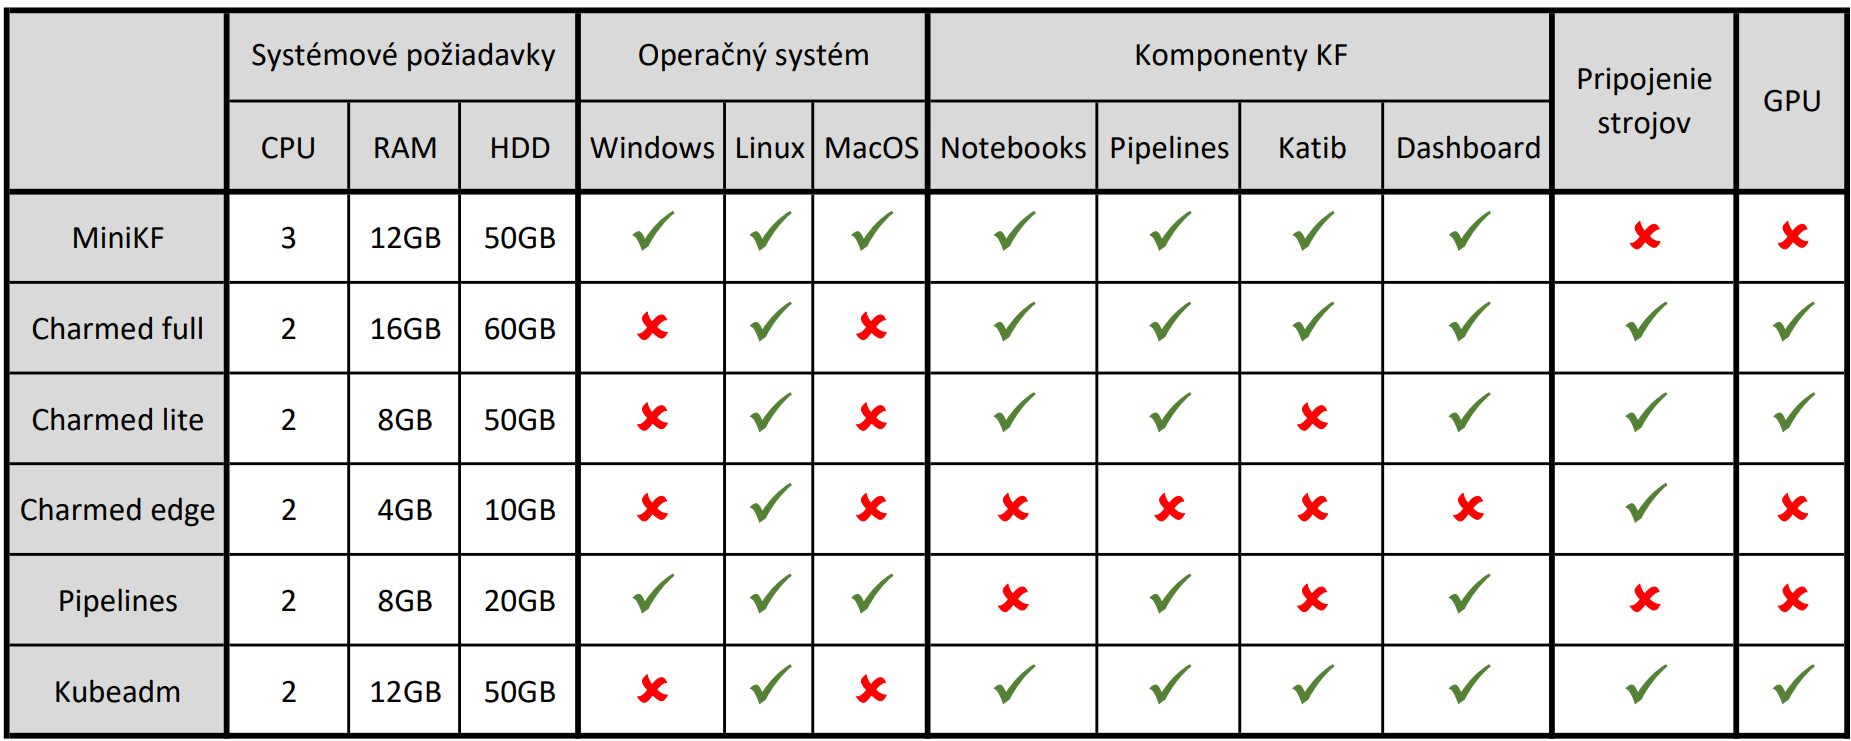
\includegraphics[width=1\linewidth]{figures/table}
    \caption{Požiadavky a funkcie implementácií.}
    \label{tab}
\end{table}